\subsection{Stima e correzione dell'offset}
\label{par2:offset}

In questa prima parte dell'esperienza tratteremo il problema dell'offset. In un amplificatore ideale sappiamo quando sia ingresso invertente che ingresso non invertente sono collegati a comune il segnale in uscita è nullo. Ciò è dovuto alla perfetta simmetria interna dell'op-amp. Ovviamente nel mondo reale non è possibile realizzare tale fatto in quanto non si riescono a costruire transistor BJT con le stesse specifiche. 

Quando colleghiamo entrambi gli ingressi a comune l'op-amp vede all'ingresso una differenza di potenziale (che ovviamente tra gli ingressi non c'è in quanto collegati entrambi a comune!) la quale viene amplificata dal guadagno a maglia aperta. Come $V_{out}$ avremo dunque un valore diverso da zero. Nel nostro caso l'op-amp andava in saturazione negativa (\SI{-12.9}{\volt}). Ricordando il funzionamento di un amplificatore operazionale, possiamo dire che il circuito si comporta come se la tensione all'ingresso invertente fosse maggiore di quella all'ingresso non invertente. Inoltre il valore $V_{out}$ è diverso dai \SI{-15}{\volt} utilizzati come alimentazione in quanto, come visto a lezione, il valore di tensione massimo $|V_{out}|$ è leggermente inferiore a $|V^-|$. In Fig.(\ref{cir:open_loop}) è riportato lo schema del circuito utilizzato.

\begin{figure}[ht]
        \centering
        \begin{subfigure}[b]{0.35\textwidth}
                 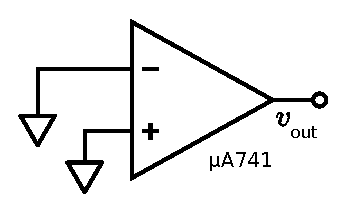
\includegraphics[width=0.70\textwidth]{../E02/latex/open_loop.pdf}
                \caption{Circuito a maglia aperta}
                \label{cir:open_loop}
        \end{subfigure}%
    \quad
        \begin{subfigure}[b]{0.35\textwidth}
               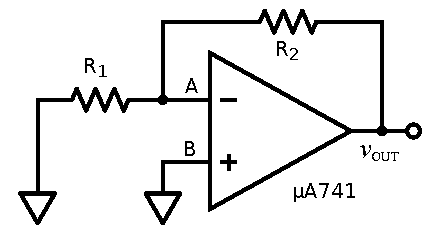
\includegraphics[width=0.70\textwidth]{../E02/latex/inv.pdf}
                \caption{Circuito amplificatore}
                \label{cir:inv}
        \end{subfigure}
     
\end{figure}

Con il circuito (\ref{cir:open_loop}) non abbiamo però una stima del valore di offset. Per fare ciò dobbiamo ricorrere a un circuito amplificatore Fig.(\ref{cir:inv}) (invertente o non invertente).

Trattiamo per primo il caso INVERTENTE. Assumiamo che la tensione nel punto A sia $V_A=V_{off}$ e $V_B=0$. L'analisi del circuito è ora banale e risulta immediatamente $V_{out}=-\frac{R_2}{R_1}V_{off}$. Ovviamente, visto che il punto A è collegato al comune, la sua tensione sarà identica a quella del punto A. La tensione $V_{off}$ è infatti un valore che concerne la struttura stessa dell'op-amp. Assumere che il punto A sia alla tensione $V_{off}$ permette dunque di analizzare il circuito. 

Ora analogamente tratteremo il caso NON INVERTENTE. per fare ciò assumiamo $V_B=-V_{off}$ e $V_A=0$. L'analisi risulta dunque identica a quella di un amplificatore non invertente, ovvero $V_{out}=(1+\frac{R_2}{R_1})V_{off}$. 

I valori nominali delle componenti circuitali utilizzate sono: $R_1=\SI{120}{\ohm}$ e $R_2=\SI{10/100}{\kilo\ohm}$.

Riportiamo nella seguente tabella i valori di offset calcolati nei due casi:

\begin{savenotes}
\begin{tabular}{c|c|c|c|c|c|c}
$R_1[\si{\ohm}]$ & $R_2[\si{\kilo\ohm}]$ & Gain(inv) & Gain (ninv) &$V_{out} [\si{\milli\volt}]$ & $V_{off}$(inv)[\si{\milli\volt}] &$V_{off}$(ninv) [\si{\milli\volt}]\\ 
\hline 
$119.8\pm0.1$ & $9.911\pm0.001$  & $-82.73\pm0.07$ &$83.73\pm0.07$&  $-103.5 \pm 0.5$ & $-1.251 \pm0.006$ & $-1.23 \pm0.01$\\
\hline
$119.8\pm0.1$ & $99.35\pm0.01$  & $-829.3\pm0.7$ & $830.3\pm0.7$ &$ -1025 \pm 2$ & $-1.236 \pm 0.002$ & $-1.2 \pm0.1$\\

\end{tabular}
\end{savenotes}

Ricordiamo che i valori di tensione di offset ottenuti per configurazione invertente e non invertente differiscono nel segno in quanto è necessario che in entrambi i casi sia rispettata la condizione $|V_{inv}|>|V_{ninv}|$.

Come sappiamo la tensione di offset non è però l'unico problema che incontriamo quando usiamo op-amp reali. Infatti ingresso invertente e non invertente sono collegati alle basi di transistor e, ovviamente, per polarizzarli serve una corrente di base. Gli effetti di tale corrente si sommeranno dunque a quelli dovuti all'offset. Tale argomento sarà comunque trattato approfonditamente nella sezione successiva. Per risolvere il problema dell'offset possiamo servirci di una resistenza variabile ($Trimmer$) che posizioneremo tra i piedini 1 e 5 dell'op-amp, collegandola a $V^-$. Regolando tale resistenza andremo a generare una contro tensione che bilancerà l'offset. 

\begin{wrapfigure}[17]{l}{0.55\textwidth}
  \begin{center}
    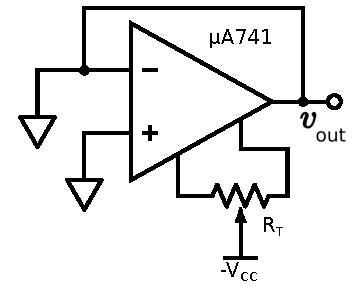
\includegraphics[width=0.30\textwidth]{../E02/latex/trimmer_correction.pdf}
  \end{center}
  \caption{Circuito con trimmer per compensare l'offset.}
  \label{cir2:trimmer}
\end{wrapfigure}

Il datasheet dell'amplificatore consiglia di utilizzare un circuito a maglia aperta senza resistenze. Tale configurazione è consigliata sia per la simmetria prima dei due ingressi (entrambi vedono la stessa impedenza $\approx 0$) sia per il fatto che il guadagno a maglia aperta molto grande ci permette praticamente di azzerare l'offset. 

Durante l'esperienza abbiamo provato ad utilizzare $Trimmer$ ad un giro da \SI{10}{\kilo\ohm} ma la sensibilità meccanica era troppo bassa per poter azzerare l'offset (la tensione di uscita infatti passava da $\approx$\SI{-13}{\volt} a $\approx$\SI{+13}{\volt}). Abbiamo dunque utilizzato un $Trimmer$ multigiro da \SI{10}{\kilo\ohm}, con il quale abbiamo raggiunto la tensione $V_{out}= (2.3\pm0.3)\si{\volt}$. Se ricordiamo che il guadagno a maglia aperta è di 100-120dB vediamo subito che siamo praticamente riusciti a bilanciare la tensione di offset.

Come già accennato le correnti di bias, per quanto piccole (\si{\nano\ampere}) giocano comunque un ruolo non indifferente sull'offset totale. Se assumiamo che $I_B^- \simeq I_B^+ $, allora basterà fare in modo che i due ingressi vedano la stessa impedenza. Così facendo il contributo delle due correnti si bilancia e abbiamo una stima più precisa dell'offset. Abbiamo dunque ripetuto le misure. Riportiamo nella seguente tabella i nuovi valori:

\begin{tabular}{c|c|c|c|c|c|c}
$R_C [\si{\ohm}]$& $R_1[\si{\ohm}]$ & $R_2[\si{\kilo\ohm}]$ & Gain (inv) & $V_{out}' [\si{\milli\volt}]$ & $V_{off}' [\si{\milli\volt}]$ & $|V_{off}-V_{off}'|[\si{\milli\volt}]$ \\ 
\hline 
$119.4\pm0.1$ & $119.8\pm0.1$ & $9.911\pm0.001$  & $-82.73\pm0.07$ & $-105.5 \pm 0.5$ & $-1.275 \pm0.006$ & $0.024\pm0.008$ \\
\hline
$119.4\pm0.1$ & $119.8\pm0.1$ & $99.35\pm0.01$  & $-829.3\pm0.7$ &$ -1038 \pm 5$ & $-1.251 \pm 0.002$ & $0.015 \pm 0.003 $	\\

\end{tabular}

Come vediamo, le differenze tra i due valori di $V_{off}$ calcolati con e senza resistenza $R_C$ sono compatibili al contributo di una corrente $I^*$ dell'ordine dei \si{\nano\ampere} che scorre nella resistenza $R_C$: $\Delta V \simeq R_C * 10^{-9} \simeq 10\div100 \si{\micro\volt}$.

Anche nel caso non invertente $\Delta V$ risulta compatibile con la caduta di potenziale data da una corrente di base di alcuni \si{\nano\ampere}.